\documentclass[10pt,a4paper, margin=1in]{article}
\usepackage{fullpage}
\usepackage{amsfonts, amsmath, pifont}
\usepackage{amsthm}
\usepackage{graphicx}

\usepackage{tkz-euclide}
\usepackage{tikz}
\usepackage{pgfplots}
\pgfplotsset{compat=1.13}

\usepackage{geometry}
 \geometry{
 a4paper,
 total={210mm,297mm},
 left=10mm,
 right=10mm,
 top=10mm,
 bottom=10mm,
 }
 % Write both of your names here. Fill exxxxxxx with your ceng mail address.
 \author{
  Baykara, Azad \\
  \texttt{e2171320@ceng.metu.edu.tr}
  \and
  Kocaman, Alper \\
  \texttt{e2169589@ceng.metu.edu.tr}
}
\title{CENG 384 - Signals and Systems for Computer Engineers \\
Spring 2018-2019 \\
Written Assignment 1}
\begin{document}
\maketitle



\noindent\rule{19cm}{1.2pt}

\begin{enumerate}

\item 
    \begin{enumerate}
    % Write your solutions in the following items.
    \item %write the solution of q1a
    \begin{align*}
    y[n] = 2x[n] + \frac{3}{4}.y[n-1] - \frac{1}{8}.y[n-2] \\
    y[n] - \frac{3}{4}.y[n-1] + \frac{1}{8}.y[n-2] = 2x[n]
    \end{align*}
    \item %write the solution of q1b
    Take Fourier Transform of the difference equation. 
    \begin{align*}
    \frac{1}{8}e^{-2jw}Y(e^{jw}) -\frac{3}{4}e^{-jw}Y(e^{jw}) + Y(e^{jw}) &= 2X(e^{jw}) \\
    Y(e^{jw}) \ . \ [\frac{1}{8}e^{-2jw} - \frac{3}{4}e^{-jw} + 1] &= 2X(e^{jw}) \\
    H(e^{jw}) &= \frac{16}{e^{-2jw} -6e^{-jw} + 8} 
    \end{align*}
    \item %write the solution of q1c
    \begin{align*}
    &H(e^{jw}) = \frac{16}{e^{-2jw} -6e^{-jw} + 8} = \frac{16}{(e^{-jw }-4)(e^{-jw} - 2)} = \frac{A}{e^{-jw }-4} + \frac{B}{e^{-jw} - 2} \\
    &A = 8 \quad B=-8 \\
    &H(e^{jw}) = \frac{8}{e^{-jw }-4} - \frac{8}{e^{-jw} - 2} \\
    &= \frac{4}{1- \frac{1}{2} e^{-jw }} - \frac{2}{1- \frac{1}{4} e^{-jw}} \\
    &Take \ inverse \ FT  \\
    &h[n] = 4(\frac{1}{2})^nu[n] -2(\frac{1}{4})^nu[n] \\
    \end{align*}
    \item %write the solution of q1d
    \begin{align*}
    Fourier \ transform \ of \ x[n] \ &= \ (\frac{1}{4})^nu[n] \ is \ \frac{1}{1-\frac{1}{4}e^{-jw}}  \\ 
    y[n] = h[n] \ast x[n] &\longleftrightarrow Y(e^{jw}) = H(e^{jw}).X(e^{jw}) \\
    Y(e^{jw}) &= (\frac{8}{e^{-jw }-4} - \frac{8}{e^{-jw} - 2}).\frac{1}{1-\frac{1}{4}e^{-jw}} \\
    &= (\frac{8}{e^{-jw }-4} - \frac{8}{e^{-jw} - 2}).\frac{4}{4-e^{-jw}} \quad let \ z = e^{-jw} \\
    &= (\frac{8}{z-4} - \frac{8}{z - 2}).\frac{4}{4-z} \\
    &= (\frac{8}{z-2} - \frac{8}{z - 4}).\frac{4}{z-4} \\
    &= \frac{32}{(z-2)(z-4)} - \frac{32}{(z - 4)^2} \\
    &= \frac{16}{z-4} - \frac{16}{z-2}- \frac{32}{(z - 4)^2} \\
    &= \frac{-4}{1-\frac{1}{4}e^{-jw}} + \frac{8}{1-\frac{1}{2}e^{-jw}}- \frac{2}{(1 - \frac{1}{4}e^{-jw})^2} \\
    Take \ inverse \ Fourier &\ transform \\
    y[n] = -4(\frac{1}{4})^nu[n] \  + \  &8(\frac{1}{2})^nu[n] \ - \ 2(n+1)(\frac{1}{4})^nu[n]
    \end{align*}
    
    \end{enumerate}


\item %write the solution of q2
If two LTI systems are connected parallel, then overall system's impulse response is 
$$ h[n] = h_1[n] + h_2[n]$$ and frequency response is $$ H(e^{jw}) = H_1(e^{jw}) + H_2(e^{jw})$$
In this question, overall system's frequeny response $H(e^{jw})$ and impulse response of first system $h_1[n]$ are given.In order to find $ h_2[n] $,\\ 
1-Frequeny response of $h_1[n]$ should be found,\\ 
2-Frequeny response of $h_2[n]$ which is $H_2(e^{jw})$ should be found using formula $$ H_2(e^{jw})\ =\ H(e^{jw})\ -\ H_1(e^{jw})$$
3-By applying inverse fourier transformation, find $h_2[n]$.\\\\

1-Frequency response of $$h_1[n]= (\frac{1}{3})^nu[n]$$ $$H_1(e^{jw}) = \frac{1}{1 - \frac{1}{3}e^{-jw}}$$ $$ H_1(e^{jw}) = \frac{-3}{e^{-jw}-3}$$
2-Frequeny response of $h_2[n]$, $$ H_2(e^{jw})\ =\ H(e^{jw})\ -\ H_1(e^{jw})$$
$$H_2(e^{jw})\ =\ \frac{5e^{-jw}-12}{e^{-2jw}-7e^{-jw}+12}\ -\ \frac{-3}{e^{-jw}-3}$$  
$$H_2(e^{jw})\ =\ \frac{5e^{-jw}-12}{(e^{-jw}-4)(e^{-jw}-3)}\ -\ \frac{-3}{e^{-jw}-3}$$ $$H_2(e^{jw})\ =\ \frac{-2}{1\ -\ \frac{1}{4}e^{-jw}} $$
3-Impulse response of $H_2(e^{jw})$ by using inverse FT, $$ h_2[n]\ =\ -2(\frac{1}{4})^nu[n] $$
\item      
    \begin{enumerate}
    \item %write the solution of q3a
    
	Input signal x(t) consists of a periodic cosine function and an aperiodic square wave which can be seperated as\\
	$$x(t)\ =\ x_1(t)\ +\ x_2(t)$$ where
	$$x_1(t)\ = \frac{sin2\pi t}{\pi t}$$   
	$$x_2(t)\ = cos3\pi t$$
	By taking fourier transformation, 
	\begin{align*}
	F\{x_1(t)\} &= X_1(jw) = \begin{cases}
                               1, & \text{if}\ |w| < 2\pi \\
                               0, & \text{otherwise}
                             \end{cases} \\ 
	\end{align*}
	$$X_2(jw)\ =\ \pi[\ \delta(\ \omega\ -\ 3\pi\ )\ +\ \ \delta(\ \omega\ +\ 3\pi\ ) ]$$	
	
	Thus, fourier transform of $x(t)$,
	$$X(jw)\ =\ X_1(jw)\ +\ X_2(jw)$$
	And the graph of $X(jw)$,
	
	\begin{figure}[h!]
    \centering
        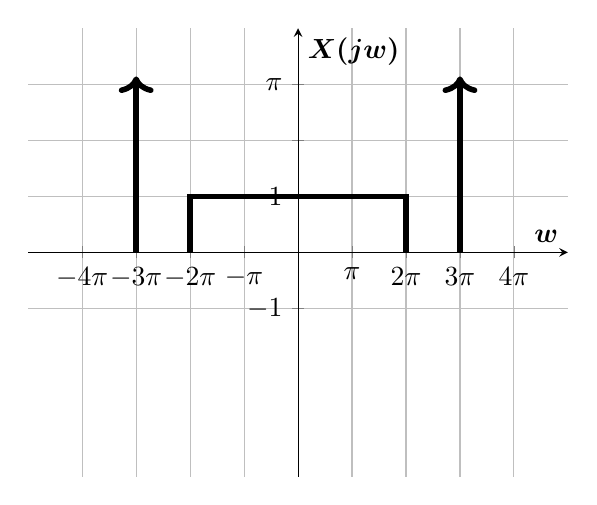
\begin{tikzpicture}[scale=1.0]
           \begin{axis}[
          axis lines=middle,
          xlabel={$\boldsymbol{w}$},
          ylabel={$\boldsymbol{X(jw)}$},
          xtick={-4, ..., 4},
          xticklabels={$-4\pi$,$-3\pi$, $-2\pi$, $-\pi$, $0$, $\pi$, $2\pi$, $3\pi$,$4\pi$},
          yticklabels={$-1$,$0$,$1$,$ $,$\pi$},
          ytick={-1,0,..., 3},
          ymin=-4, ymax=4,
          xmin=-5, xmax=5,
          grid,
        ]
           \path[draw,line width=2pt] (-2,0) -- (-2,1) -- (2,1) -- (2,0);
           \draw[->, line width=2pt] (-3, 0) -- (-3, 3.14);
           \draw[->, line width=2pt] (3, 0) -- (3, 3.14);
           \end{axis}
        \end{tikzpicture}
        \caption{$w$ vs. $X(jw)$.}
        \label{fig:q2}
    \end{figure}
	 
    \item %write the solution of q3b
    
    From part a), Nyquist frequency is $3\pi$.\\ Since $$ w_s = 2\times w_m$$ $$ w_s = 6\pi$$ Nyquist rate is $6\pi$.\\Sampling rate is $$T\ =\ \frac{2\pi}{6\pi}\ =\ \frac{1}{3} $$
    
    \item %write the solution of q3c
    
    By using formula,
    $$ X_p(jw)\ =\ \frac{1}{T} \sum_{k =\ -\infty} ^{\infty}X(j(\omega\ -\ k\omega_s))$$
    $$ X_p(jw)\ =\ 3 \sum_{k =\ -\infty} ^{\infty}X(j(\omega\ -\ 6\pi k))$$
    
    (Graph of this question is below, top of the next page) 
    
    \begin{figure}[h!]
    \centering
        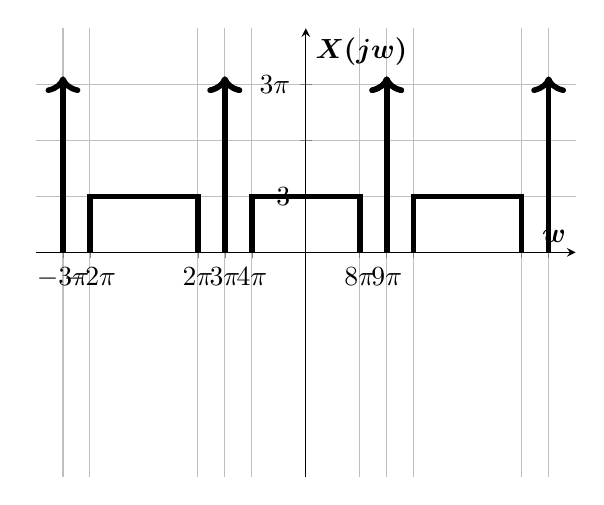
\begin{tikzpicture}[scale=1.0]
           \begin{axis}[
          axis lines=middle,
          xlabel={$\boldsymbol{w}$},
          ylabel={$\boldsymbol{X(jw)}$},
          xtick={-9,-8,-4,-3,-2,2,3,4,8,9},
          xticklabels={$-3\pi$, $-2\pi$, $2\pi$, $3\pi$, $4\pi$, $8\pi$, $9\pi$ },
          yticklabels={$0$,$3$,$ $ , $3 \pi$},
          ytick={0,..., 3},
          ymin=-4, ymax=4,
          xmin=-10, xmax=10,
          grid,
        ]
           \path[draw,line width=2pt] (-2,0) -- (-2,1) -- (2,1) -- (2,0);
           \draw[->, line width=2pt] (-3, 0) -- (-3, 3.14);
           \draw[->, line width=2pt] (3, 0) -- (3, 3.14);
           
           \path[draw,line width=2pt] (4,0) -- (4,1) -- (8,1) -- (8,0);
           \draw[->, line width=2pt] (3, 0) -- (3, 3.14);
           \draw[->, line width=2pt] (9, 0) -- (9, 3.14);
           
           \path[draw,line width=2pt] (-4,0) -- (-4,1) -- (-8,1) -- (-8,0);
           \draw[->, line width=2pt] (-3, 0) -- (-3, 3.14);
           \draw[->, line width=2pt] (-9, 0) -- (-9, 3.14);
           
           
           \end{axis}
        \end{tikzpicture}
        \caption{$w$ vs. $X(j(w-6\pi k))$.}
        \label{fig:q3}
    \end{figure}
    
    \end{enumerate}

\item 
    \begin{enumerate}
    \item %write the solution of q4a
    \begin{align*}
    N &= \frac{2\pi}{w_s} = 2 \\
    X_p(jw) &= \frac{1}{T} \sum_{\forall k}X(j(w-kw_s)) \\
    X_d(e^{jw}) &= X_p(j\frac{w}{T})  \\ 
    X_d(e^{jw}) &= 
    \begin{cases} 
      \frac{2}{\pi}w & if \ | w | \leq \frac{\pi}{2} \\
      0 & otherwise
    \end{cases} \quad \ ,X_d(e^{jw}) = X_d(e^{j(w+N)})
    \end{align*}

    \item %write the solution of q4b
    From discrete time Fourier transform table, we know that
    \begin{align*}
    e^{jw_0n} & \longleftrightarrow 2\pi \sum_{\forall k} \delta(w-w_0-2\pi k) \\
    h[n] &= cos\pi n = \frac{1}{2} (e^{j\pi n} + e^{-j\pi n}) \\
    Then, \ H(e^{jw}) &= \frac{1}{2} (2\pi \sum_{\forall k} \delta(w-\pi-2\pi k) + 2\pi \sum_{\forall k} \delta(w+\pi-2\pi k)) \\
    &= \pi (\sum_{\forall k} \delta(w-\pi-2\pi k) + \delta(w+\pi-2\pi k))
    \end{align*}
    \item %write the solution of q4c
    \begin{align*}
    &y_d[n] = x_d[n].h[n] \longleftrightarrow Y_d(e^{jw}) = \frac{1}{2\pi} X_d(e^{jw})*H(e^{jw}) \\
    &Convolution \ over \ 1 \ period \ (-\pi \ to \ \pi) \\
    &Y_d(e^{jw}) = \frac{1}{2\pi}.\pi (\sum_{\forall k} \delta(w-\pi) + \delta(w+\pi))\ast X_d(e^{jw}) \\
    &Shift \ X_d(e^{jw}) \ to \ the \ left \ and \ right \ by \ \pi. \ Hence, \\    
    Y_d(e^{jw}) &= 
    \begin{cases} 
      \frac{1}{\pi}w & , \ \frac{\pi}{2} \leq | w | \leq \frac{3\pi}{2} \\
      0 & otherwise
    \end{cases} \quad \ ,Y_d(e^{jw}) = X_d(e^{j(w+2\pi)})
    \end{align*}
    \end{enumerate}


\end{enumerate}
\end{document}

